% SIAM UQ Supplementary Materials
\documentclass[supplement,review,hidelinks,onefignum,onetabnum]{siamart251216}

\usepackage{amsmath,amssymb}
\usepackage{mathtools}
\usepackage{bm}
\usepackage{graphicx}
\usepackage{booktabs}
\usepackage{enumitem}
\usepackage{algorithm}
\usepackage{algpseudocode}
\usepackage{xr-hyper}
\usepackage{xcolor}
\externaldocument[M-]{part1_method}

\newcommand{\RR}{\mathbb{R}}
\newcommand{\NN}{\mathbb{N}}
\newcommand{\EE}{\mathbb{E}}
\newcommand{\PP}{\mathbb{P}}
\newcommand{\Var}{\mathrm{Var}}
\newcommand{\Cov}{\mathrm{Cov}}
\newcommand{\tr}{\operatorname{Tr}}
\newcommand{\DKL}{\mathcal{D}_{\mathrm{KL}}}
\newcommand{\diag}{\mathrm{diag}}
\newcommand{\divop}{\operatorname{div}}
\DeclareMathOperator*{\argmin}{arg\,min}
\DeclareMathOperator*{\argmax}{arg\,max}
\newcommand{\gauss}{\gamma}
\renewcommand{\vec}[1]{\bm{#1}}
\newcommand{\mA}{\bm{A}}
\newcommand{\mb}{\bm{b}}
\newcommand{\mh}{\bm{h}}
\newcommand{\mC}{\bm{C}}
\newcommand{\hmC}{\widehat{\bm{C}}}
\newcommand{\mV}{\bm{V}}
\newcommand{\hmV}{\widehat{\bm{V}}}
\newcommand{\mP}{\bm{P}}
\newcommand{\hPperp}{\widehat{\mP}_{\perp}^{\mC}}
\newcommand{\hmP}{\widehat{\bm{P}}}
\newcommand{\mS}{\bm{S}}
\newcommand{\mPsi}{\bm{\Psi}}
\newcommand{\mU}{\bm{U}}
\newcommand{\mR}{\bm{R}}
\newcommand{\mD}{\bm{D}}
\newcommand{\mH}{\bm{H}}
\newcommand{\mL}{\bm{L}}
\newcommand{\mM}{\bm{M}}
\newcommand{\mI}{\bm{I}}
\newcommand{\mW}{\bm{W}}
\newcommand{\mG}{\bm{G}}
\newcommand{\mQ}{\bm{Q}}
\newcommand{\mSigma}{\bm{\Sigma}}
\newcommand{\vzero}{\bm{0}}
\newcommand{\cond}{\operatorname{cond}}
\newcommand{\vx}{\bm{x}}
\newcommand{\vy}{\bm{y}}
\newcommand{\vn}{\bm{n}}
\newcommand{\vz}{\bm{z}}
\newcommand{\vZ}{\bm{Z}}
\newcommand{\vu}{\bm{u}}
\newcommand{\vU}{\bm{U}}
\newcommand{\vY}{\bm{Y}}
\newcommand{\vv}{\bm{v}}
\newcommand{\vw}{\bm{w}}
\newcommand{\vtheta}{\bm{\theta}}
\newcommand{\whvtheta}{\widehat{\bm{\theta}}}
\newcommand{\scL}{\mathcal{L}}
\newcommand{\scZ}{\mathcal{Z}}
\newcommand{\scS}{\mathcal{S}}
\newcommand{\scF}{\mathcal{F}}
\newcommand{\St}{\mathrm{St}}
\newcommand{\Gr}{\mathrm{Gr}}

% Additional macros used in moved appendices (App E, F, G)
\newcommand{\hbeta}{\widehat{\beta}}
\newcommand{\vW}{\bm{W}}
\newcommand{\veta}{\bm{\eta}}
\newcommand{\vb}{\bm{b}}
\newcommand{\va}{\bm{a}}
\newcommand{\ve}{\bm{e}}
\DeclareMathOperator{\range}{range}
\newcommand{\hmA}{\widehat{\bm{A}}}
\newcommand{\hmM}{\widehat{\bm{M}}}
\newcommand{\hmb}{\widehat{\bm{b}}}
\newcommand{\mB}{\bm{B}}
\newcommand{\hvbeta}{\widehat{\bm{\theta}}^{r}}

\setlength{\emergencystretch}{3em}
\newcommand{\creflastconjunction}{, and~}

\newsiamremark{remark}{Remark}
\newsiamremark{assumption}{Assumption}
\crefname{remark}{Remark}{Remarks}
\crefname{assumption}{Assumption}{Assumptions}
% Cleveref types labels in \newsiamremark environments by the shared theorem
% counter, so \Cref of a remark or assumption prints "Theorem N". Alias the
% counter to the correct type inside each environment (the alias is local to
% the environment group), which makes \Cref print Remark/Assumption.
\let\origremarkenv\remark
\renewcommand{\remark}{\crefalias{theorem}{remark}\origremarkenv}
\let\origassumptionenv\assumption
\renewcommand{\assumption}{\crefalias{theorem}{assumption}\origassumptionenv}

\headers{Copula Active Subspaces}{J.~Chen and P.~J.~van Leeuwen}
\title{Copula Active Subspaces I: A Score-Covariance Method for Reduced-Order Non-Gaussian Density Estimation\thanks{Submitted to the editors \today. \funding{This work was supported by the Consortium for Advanced Data Assimilation Research and Education (CADRE), funded by NOAA under grant 2007893.}}}
\author{%
  Joshua Chen\thanks{Department of Atmospheric Science, Colorado State University, Fort Collins, CO 80523 (\email{Joshua.Chen@colostate.edu}).}
  \and
  Peter Jan van Leeuwen\thanks{Department of Atmospheric Science, Colorado State University, Fort Collins, CO 80523 (\email{Peter.vanLeeuwen@colostate.edu}).}
}

\begin{document}
\maketitle

These supplementary materials carry the empirical support and the optional methodological extensions of Part~I.
\begin{itemize}
\item \Cref{sm:rate-real} measures the dependence of Stage-1 subspace recovery on $(K_1, q_1)$, reports the PCA subspace baseline on Example~1 and the Bayesian inference problem, compares subspaces with Stage-2 estimation removed, and measures the accuracy of the tail-sum diagnostic $\widehat E_r$ against a numerical reference.
\item \Cref{sm:s2reg-empirical} compares the Stage-2 regularizer $\mR$ across the coefficient $C$, specifies the validation choice of the two constants and the centering constraint, and sets $\mR$ against $\mR_{H^2}$ at the best $\kappa$ chosen separately for each $N$, on all three examples.
\item \Cref{sm:adaptivity} describes an optional greedy choice of the Stage-1 degree and interaction order using reusable quadratic solves, with its costs and the meaning of its stopping rule.
\item \Cref{sm:marginals} identifies the marginals of the reduced model, states the reductions under which they are preserved, and bounds their deviation.
\end{itemize}
Throughout, $\vn$ denotes the observation noise in its original (pre-rank-transform) coordinates, with law $\pi_{\vn}$, and all other notation follows the main manuscript. Numbers carrying the SM prefix (\S\ref{sm:rate-real}, \Cref{tab:pca-banana}, \eqref{eq:subspace-only-kl}) refer to these supplementary materials, and numbers without it refer to the main manuscript.


% =====================================================================
\section{Stage-1 subspace convergence and PCA subspace baseline}
\label{sm:rate-real}

This section provides additional numerical support for the Stage-1 results of the main manuscript: the dependence of Stage-1 subspace recovery on $(K_1, q_1)$, and the per-$(r, N)$ numbers behind the PCA baseline of \S\ref{M-sec:exp-testll}.


On the examples of \S\ref{M-sec:exp-benchmark} the copula score need not be represented exactly by a fixed Hermite multi-index set, which does not by itself imply a subspace error (\Cref{M-lem:pilot-subspace}). Main-paper \Cref{M-fig:recovery-row} measures the combined effect of the multi-index set, the Stage-1 penalty and sampling against the reference $\mV_r^{\mC}$ at $N_{\rm ref} = 10^6$, at the multi-index sets the cross-validation criterion chooses; the angle is smaller where a richer set is chosen. The score-covariance spectra of the three example problems appear side by side in \Cref{fig:eigvals-all}, with Example~1 in the left panel.

\begin{figure}[h]
\centering
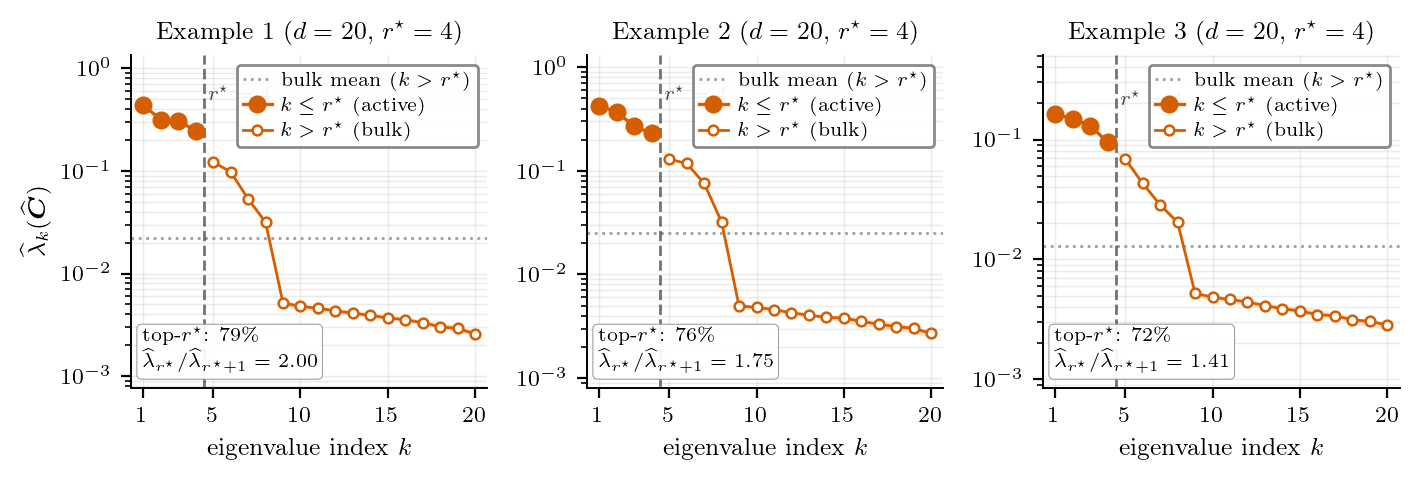
\includegraphics[width=\textwidth]{eigvals_all.png}
\caption{Eigenvalue decay of the \emph{estimated} copula-score covariance $\hmC$ is shown on the three example problems at $N=50{,}000$ and the Stage-1 multi-index set $(K_1, q_1) = (4,2)$, as the median across five realizations with the band spanning their range, and with Example~1 in the left panel, Example~2 in the middle, and Example~3 on the right. Filled markers are the top-$r^\star$ eigenvalues, hollow markers the remaining $k > r^\star$, the dashed vertical line $r^\star = 4$, and the dotted horizontal line the mean of the eigenvalues above $r^\star$. These are eigenvalues of $\hmC$, which is assembled from the parameterized score at a coarse multi-index set and is accordingly smaller in scale than the reference $\mC$ whose spectrum \S\ref{M-sec:exp-benchmark} quotes. The panels show the shape of the decay and the gap at $r^\star$.}
\label{fig:eigvals-all}
\end{figure}

\subsection*{PCA subspace baseline: per-$(r, N)$ numbers}\label{sec:pca-ablation}

We compare \textsc{Cas} with the PCA baseline of \S\ref{M-sec:exp-testll}. The two share everything but the subspace: the rank transform, the Stage-2 estimate on the projected coordinates, and the evaluation. \textsc{Cas} uses $\hmV_r^{\mC}$, the top-$r$ eigenvectors of $\hmC$; PCA uses $\hmV_r^{\widehat\Sigma}$, those of the ordinary covariance $\widehat\Sigma$ on the rank-Gaussianized data. This comparison sweeps $r \in \{2, 3, 4, 6, 8\}$ at $N \in \{500, 1000, 2000\}$ over $20$ independent realizations, and evaluates each estimate on a fifth of its own sample withheld from the estimate rather than on the independent sample of \S\ref{M-sec:exp-testll}.

\paragraph{Example~1 noise law (\S\ref{M-sec:exp-banana})} \Cref{tab:pca-banana} summarizes the out-of-sample log-likelihood at each $(r, N)$ pair. PCA is flat across $r \in \{2, \ldots, 8\}$ for each $N$ (mean out-of-sample log-likelihood $\approx -40.41$ at $N = 1000$, $\approx -40.29$ at $N = 2000$): adding rank does not help, because PCA's variance directions miss the non-Gaussian dependence. \textsc{Cas} is better in $12$ of the $15$ pairs and within the $0.05$-nat margin in the other three, all at $N = 500$; the gap reaches $\approx 0.35$ nats for $r = 6$ at $N = 2000$ and increases with $N$ in every row. At ranks $6$ and $8$ the Stage-2 solve of \Cref{M-app:solver} reaches its round cap with the level bound unmet in $40$ and $70$ of the $120$ fits, respectively, and none at ranks $2$--$4$; those fits keep the solver's last iterate.

\begin{table}[h]
\centering\footnotesize
\setlength{\tabcolsep}{4pt}
\caption{Mean out-of-sample log-likelihood on Example~1 ($d = 20$) is reported over $20$ independent realizations. Bold marks the better estimator at each $(r, N)$ pair ($\geq 0.05$-nat margin). \textsc{Cas} is better in $12$ of the $15$ pairs; the other three, at $N = 500$ for $r \in \{2, 3, 8\}$, are within the margin.}
\label{tab:pca-banana}
\begin{tabular}{r|rr|rr|rr}
\toprule
& \multicolumn{2}{c|}{$N{=}500$} & \multicolumn{2}{c|}{$N{=}1000$} & \multicolumn{2}{c}{$N{=}2000$} \\
$r$ & \textsc{Cas} & PCA & \textsc{Cas} & PCA & \textsc{Cas} & PCA \\
\midrule
2  & $-40.71$ & $-40.75$ & $\mathbf{-40.34}$ & $-40.41$ & $\mathbf{-40.22}$ & $-40.29$ \\
3  & $-40.70$ & $-40.75$ & $\mathbf{-40.26}$ & $-40.41$ & $\mathbf{-40.11}$ & $-40.30$ \\
4  & $\mathbf{-40.68}$ & $-40.74$ & $\mathbf{-40.19}$ & $-40.41$ & $\mathbf{-39.99}$ & $-40.29$ \\
6  & $\mathbf{-40.67}$ & $-40.73$ & $\mathbf{-40.17}$ & $-40.40$ & $\mathbf{-39.94}$ & $-40.29$ \\
8  & $-40.68$ & $-40.72$ & $\mathbf{-40.20}$ & $-40.39$ & $\mathbf{-39.95}$ & $-40.28$ \\
\bottomrule
\end{tabular}
\end{table}

\paragraph{Inference-problem example (\S\ref{M-sec:exp-bip})} On the Bayesian inference problem at $N = 50{,}000$, PCA does not reduce the posterior KL divergence by more than $3\%$ at any rank: its mean KL divergence ($0.45$--$0.46$ across $r \in \{2, \ldots, 8\}$) differs by at most $0.013$ from the Gaussian-copula baseline ($0.46$), because the variance-ranked subspace does not contain the score-covariance directions. \textsc{Cas} for $r = 4$ reduces the KL divergence by $50\%$ (mean $0.23$ versus $0.46$). The gap is the contribution of the score-covariance subspace alone, since the two estimators differ in nothing else: PCA-HCSM can represent non-Gaussian dependence, but only within a subspace ranked by variance, and that subspace does not contain the directions along which the copula varies.

\begin{table}[h]
\centering\footnotesize
\caption{The Bayesian inference problem under the Example~1 noise law is evaluated over $30$ observations at $N = 50{,}000$, a separate run from the comparison of \S\ref{M-sec:exp-bip}: each estimator is computed once and held fixed, so the variation across trials comes from the observation alone. PCA improves on the Gaussian baseline by at most $3\%$ at any $r$, while \textsc{Cas} at $r = 4$ reduces the KL divergence by $50\%$.}
\label{tab:pca-bip}
\begin{tabular}{lcccc}
\toprule
Method & mean $\DKL$ & median $\DKL$ & worst $\DKL$ & reduction vs.\ Gauss \\
\midrule
Gaussian            & $0.46$ & $0.34$ & $1.38$ & n/a \\
Product of marginals & $0.46$ & $0.34$ & $1.38$ & $0\%$ \\
PCA, $r=2$  & $0.46$ & $0.34$ & $1.37$ & $0\%$ \\
PCA, $r=3$  & $0.46$ & $0.35$ & $1.37$ & $-1\%$ \\
PCA, $r=4$  & $0.46$ & $0.35$ & $1.37$ & $-1\%$ \\
PCA, $r=6$  & $0.46$ & $0.33$ & $1.37$ & $0\%$ \\
PCA, $r=8$  & $0.45$ & $0.33$ & $1.35$ & $3\%$ \\
\textsc{Cas}, $r=4$ & $\mathbf{0.23}$ & $\mathbf{0.17}$ & $\mathbf{0.96}$ & $\mathbf{50\%}$ \\
\bottomrule
\end{tabular}
\end{table}

\paragraph{Interpretation} The comparison isolates the choice of subspace: \textsc{Cas} and PCA-HCSM share the rank transform, the Stage-2 estimate, and the evaluation, so the difference between them is what identifying $\mV_r$ from the score covariance adds over identifying it from the ordinary covariance. That difference reaches $\approx 0.35$ nats of out-of-sample log-likelihood on Example~1's noise law ($r = 6$, $N = 2000$), and a $50\%$ KL divergence reduction on the inference problem, against at most $3\%$ for PCA at any rank.

\subsection*{Subspace-only KL divergence: the reduction with Stage 2 removed}
\label{sec:subspace-only-kl}

The comparisons above and in \S\ref{M-sec:exp-testll} evaluate the full estimator, so the subspace and the Stage-2 estimate contribute together. This comparison removes Stage-2 estimation entirely and compares subspaces alone. For a candidate $\mV_r$ we evaluate
\begin{equation}
  D_{\mathrm{KL}}\bigl(\pi_{\vZ}\,\|\,\pi_{\vZ}(\,\cdot\,;\mV_r)\bigr) \;=\; \EE_{\pi_{\vU}}\bigl[D_{\mathrm{KL}}(\pi_{\vW\mid\vU}\,\|\,\gauss_{d-r})\bigr],
  \label{eq:subspace-only-kl}
\end{equation}
the divergence the reduction alone incurs when the reduced density on that subspace is exact, as in \S\ref{M-sec:reduced-form} of the main manuscript. \Cref{fig:random-subspace} reports it on the three examples for $\mV_r$ estimated by \textsc{Cas}, by PCA, and drawn uniformly at random. The \textsc{Cas} divergence decreases with $N$ toward its value at the reference $\mV_r^{\mC}$ on all three. The PCA divergence does not decrease, and lies within the spread of the uniformly random draws, as \S\ref{M-sec:exp-banana} leads one to expect: the latent construction leaves no covariance structure that distinguishes the active directions.

\begin{figure}[h]
\centering
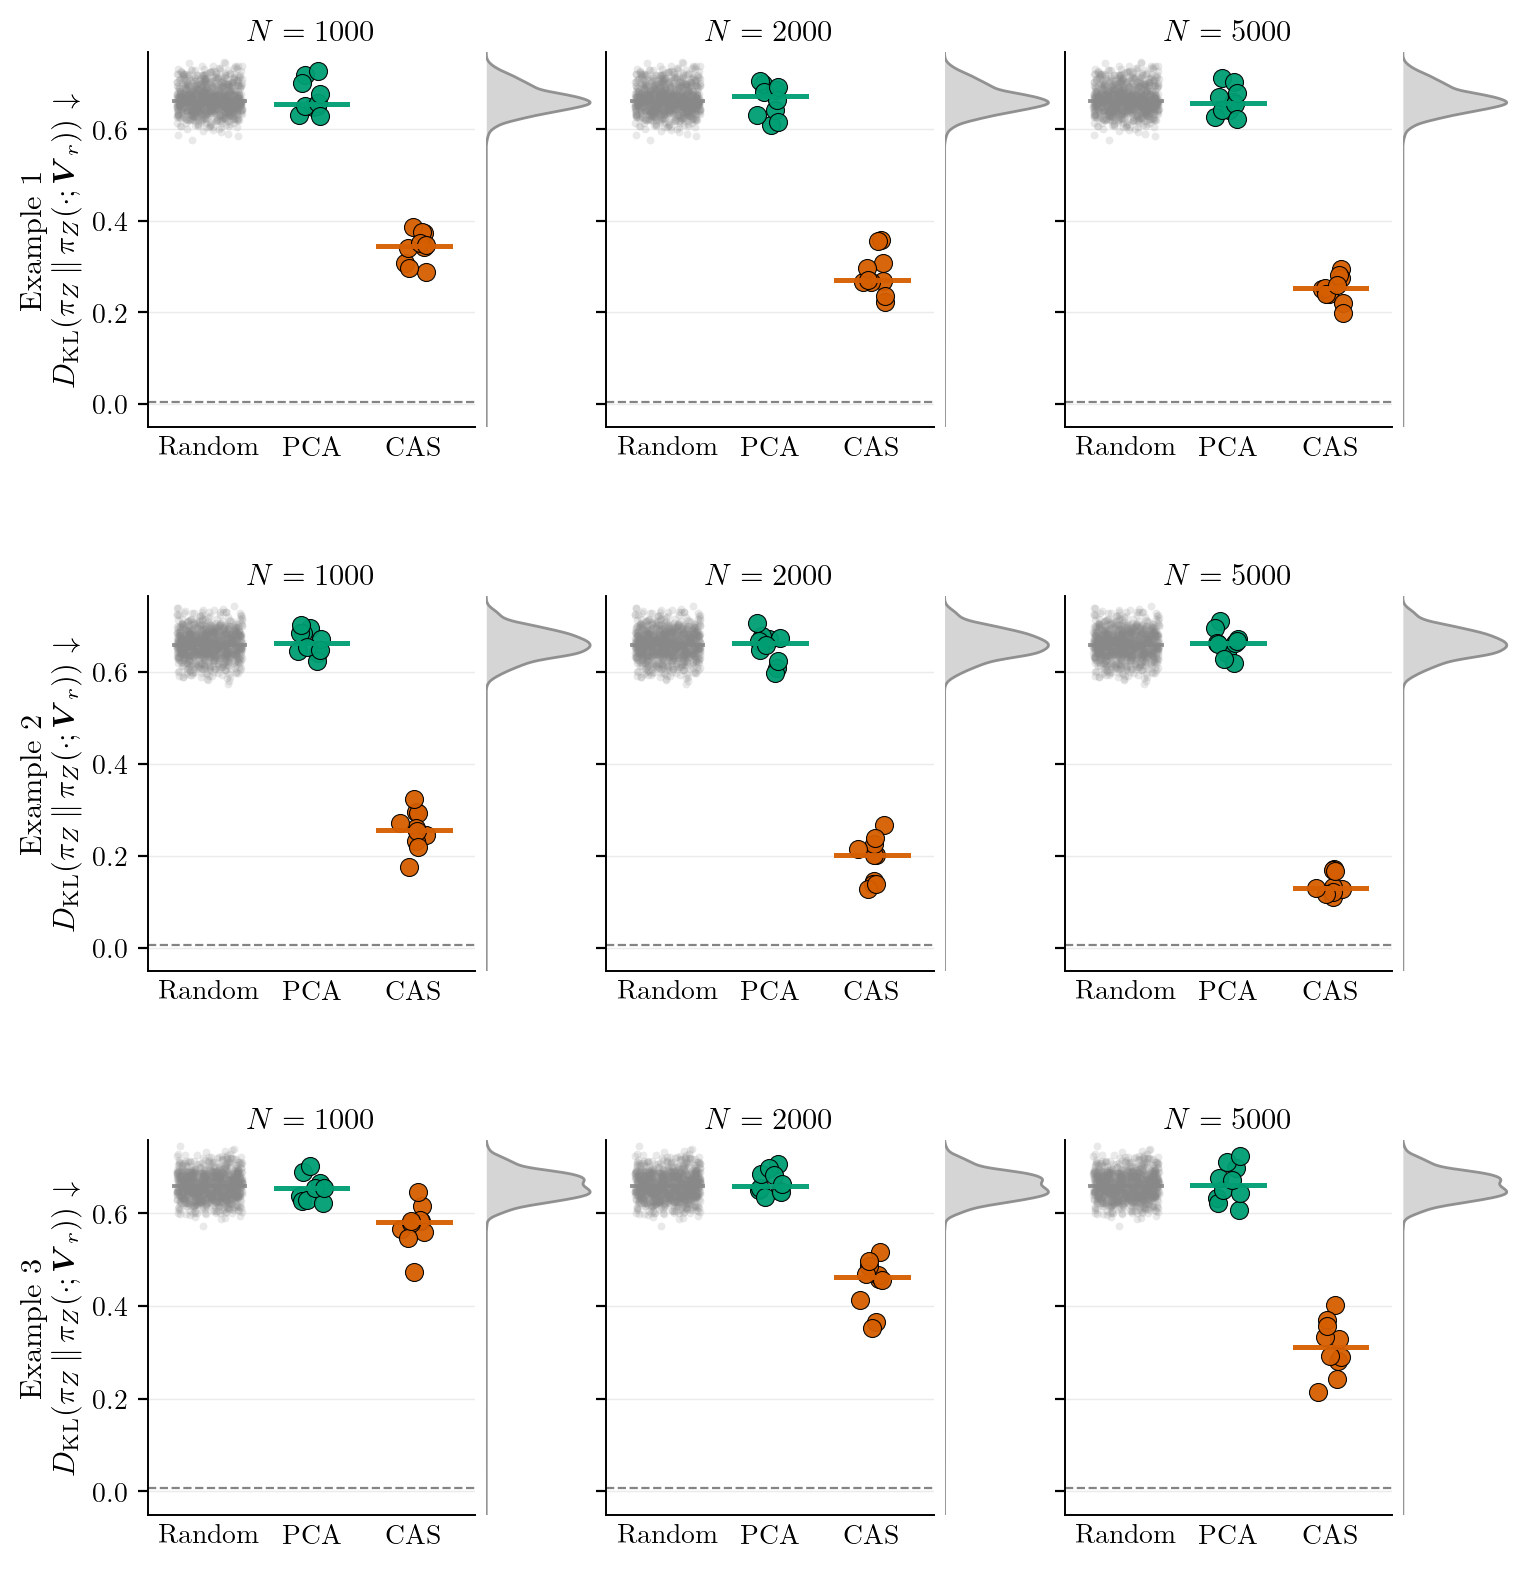
\includegraphics[width=\textwidth]{random_subspace.png}
\caption{The subspace-only KL divergence \eqref{eq:subspace-only-kl} across the three examples compares the choice of subspace with Stage-2 estimation removed, and lower is better. The gray cloud shows $J=100$ uniformly random subspaces in each of the $10$ realizations, the green markers show PCA, the orange markers show \textsc{Cas}, and the dashed line marks the value at the reference $\mV_r^{\mC}$. The \textsc{Cas} divergence decreases with $N$ toward it on all three examples, while the PCA divergence does not decrease and lies within the random-subspace cloud.}
\label{fig:random-subspace}
\end{figure}

The estimate of \eqref{eq:subspace-only-kl} is nested Monte Carlo with outer size $N_{\mathrm{outer}} = 1500$ and inner size $M_{\mathrm{inner}} = 4096$, with the copula density evaluated through marginal estimates fitted on $2\times10^6$ samples, for $N \in \{1000, 2000, 5000\}$ with $10$ independent realizations at each $N$. The uniformly random subspaces are spanned by $\mV_r^{\mathrm{rand}} = \mathrm{QR}(\mG)$ with $\mG \sim \gauss^{d\times r}$, whose column space is uniform on $\Gr(r,\RR^d)$ \cite{Mezzadri2007}, drawn independently for each realization.

\subsection*{Accuracy of the tail-sum diagnostic}
\label{sec:ehat-tightness}

\Cref{M-prop:diagnostic} bounds the error of the tail sum $\widehat E_r$ by the singular values $\sigma_j$ of the error of $\hmC$, $|\widehat E_r - E_r(\mC_\Lambda)| \le \sum_{j\le d-r}\sigma_j(\hmC - \mC_\Lambda) \le (d-r)\,\|\hmC - \mC_\Lambda\|_{\rm op}$ (\Cref{M-eq:Ehat-weyl}), and the same inequalities hold with any symmetric matrix in place of $\mC_\Lambda$. \Cref{tab:ehat-tightness} evaluates them against a numerical reference $\mC_{\rm ref}$, the score second-moment matrix at the Stage-1 coefficients fitted at $N_{\rm ref} = 10^6$, which carry the penalty of \eqref{M-eq:tikhonov}, evaluated by Monte Carlo on $2\times10^5$ fresh samples; its error column measures disagreement with that reference, not with $\mC_\Lambda$. It reports, per example at $N = 50{,}000$ over $20$ independent realizations, at the Stage-1 multi-index set $(K_1, q_1) = (4, 2)$ of the main experiments and rank $r = 4$: the sample tail sum $\widehat E_r$, the reference value $E_r(\mC_{\rm ref})$, the largest error $\max_s |\widehat E_r - E_r(\mC_{\rm ref})|$ across realizations, the across-realization means of $\sum_{j\le d-r}\sigma_j$ and of $(d-r)\,\sigma_1$, and the across-realization mean of the per-realization ratio of the first bound to the error.

\begin{table}[h]
\centering\small
\setlength{\tabcolsep}{3pt}
\caption{The accuracy of the tail-sum diagnostic and the tightness of \Cref{M-eq:Ehat-weyl} are reported per example at $N = 50{,}000$ with $20$ independent realizations, at the Stage-1 multi-index set $(K_1,q_1) = (4,2)$ of the main experiments and rank $r = 4$. Columns give the tail sum $\widehat E_r$ (mean $\pm$ one standard deviation across realizations), the reference $E_r(\mC_{\rm ref})$, the largest error across realizations, the across-realization means of the two bounds of \Cref{M-eq:Ehat-weyl}, $\sum_{j\le d-r}\sigma_j(\hmC-\mC_{\rm ref})$ and $(d-r)\,\sigma_1(\hmC-\mC_{\rm ref})$, and the mean per-realization ratio of the first bound to the error.}
\label{tab:ehat-tightness}
\begin{tabular}{l|cccccc}
\toprule
 & $\widehat E_r$ & $E_r(\mC_{\rm ref})$ & $\max_s|\widehat E_r - E_r(\mC_{\rm ref})|$ & $\sum_{j\le d-r}\sigma_j$ & $(d{-}r)\,\sigma_1$ & ratio \\
\midrule
Example~1 & $0.3490 \pm 0.0061$ & $0.2884$ & $0.0729$ & $0.1118$ & $0.3498$ & $1.9$ \\
Example~2 & $0.3994 \pm 0.0063$ & $0.3388$ & $0.0691$ & $0.1168$ & $0.3470$ & $1.9$ \\
Example~3 & $0.2058 \pm 0.0045$ & $0.1483$ & $0.0664$ & $0.0823$ & $0.2083$ & $1.4$ \\
\bottomrule
\end{tabular}
\end{table}

The ratio column is the factor by which the first bound of \Cref{M-eq:Ehat-weyl} exceeds the error it bounds. The error $\widehat E_r - E_r(\mC_{\rm ref}) = \sum_{i>r}(\widehat\lambda_i - \lambda_i(\mC_{\rm ref}))$ is a signed sum of $d-r$ eigenvalue differences, while the first bound sums the $d-r$ largest singular values of $\hmC-\mC_{\rm ref}$ without signs, and the second replaces every singular value by the largest. The two bound columns thus separate the slack from sign cancellation and the slack from the uniform norm.

\Cref{tab:ehat-tightness} shows three things. First, the error is one-signed: $\widehat E_r > E_r(\mC_{\rm ref})$ on every realization of every example. Second, the Ky Fan bound \cite{Bhatia1997} exceeds the realized error by mean factors of $1.9$, $1.9$ and $1.4$ on Examples~1--3 (the ratio column). Third, the operator-norm bound $(d-r)\,\sigma_1$ exceeds $E_r(\mC_{\rm ref})$ itself on all three examples: at $d - r = 16$ that form of \Cref{M-eq:Ehat-weyl} is uninformative here, and only the Ky Fan form is informative. The measured error is the error column and is smaller than either bound.


% =====================================================================
\section{\texorpdfstring{Stage-2 regularizer: empirical comparisons across $C$}{Stage-2 regularizer: empirical comparisons across C}}
\label{sm:s2reg-empirical}

The invariance of the Stage-2 regularizer $\mR$ to the choice of basis and its conditioning bound are established in \S\ref{M-sec:ridge} of the main paper, its Fisher divergence error bound in the companion analysis \cite{CAS_partII}, and the Stage-2 score-matching foundations in Appendix~\ref{M-app:stage2-foundations} of the main paper. This section provides additional numerical support for the Stage-2 regularizer of \S\ref{M-sec:ridge} as the default: a comparison across the coefficient $C$, and a direct comparison of $\mR$ against $\mR_{H^2}$ with the best $\kappa$ chosen separately for each $N$. The comparisons in \S\ref{sec:sm2-tr-ablations}--\ref{sec:sm2-dw-vs-h} are against $\mR_{H^2}$ on Example~1, and \S\ref{sec:sm-cross-benchmark} compares $\mR$ with alternative designs on all three examples. The Stage-2 solves in this section are the centered closed form \eqref{M-eq:stage2-closedform}, without the inequality constraints of \Cref{M-app:solver} and with the fitted potential capped above at evaluation. For noise estimates the compared quantities are the held-out log-likelihood $\EE_{\pi_{\vn}}[\log q]$ and log-score $\EE_{\pi_{\vn}}[\log\pi_{\vn} - \log q]$, where $q$ is the estimate normalized by a $2^{13}$-point reduced normalizer alone rather than by $\widehat Z_{\vn}$ of \eqref{M-eq:cas-estimator}; each differs from its normalized counterpart by the estimate's log-mass, and a paired difference by the difference of two log-masses. Posterior divergences are normalized on the grid.

\subsection{Choice of the two constants}
\label{sec:sm2-selection}
The two constants $(C_{\rm samp}, C_{\rm curv})$ of \S\ref{M-sec:ridge} are chosen from the sample by cross-validation, with no hand-tuning and no reference density. The Stage-2 sample is partitioned into an estimation part and a validation part, and the score-matching quadratic of \S\ref{M-sec:ridge} is assembled on each part. For each candidate pair on the $5\times5$ grid of \Cref{M-app:protocol}, the estimator is solved on the estimation part and scored by the validation quadratic. The minimizing pair is chosen, and the estimator is re-estimated on the full sample at the chosen values. For fixed coordinates and a candidate fitted without the validation observations, the validation quadratic estimates the reduced Fisher divergence up to a candidate-independent constant; here the transform and the subspace are estimated before the split, so we use it as an empirical tuning criterion, which requires no normalizer and no noise model. The pair $(C_{\rm samp}, C_{\rm curv}) = (3, 10^{-5})$ is the center of that grid and the fixed pair at which the comparisons of \Cref{sec:sm2-tr-ablations,sec:sm2-dw-vs-h} hold the proposal.

\subsection{\texorpdfstring{Stage-2 coefficient $C$: stability and margin over $\mR_{H^2}$}{Stage-2 coefficient C: stability}}
\label{sec:sm2-tr-ablations}

We assess the stability of the Stage-2 coefficient $C := C_{\rm samp}$ and the margin of $\mR$ over $\mR_{H^2}$ on Example~1 of \S\ref{M-sec:exp-banana}. Holding the subspace, rank, and marginals fixed, we compare $\mR$ for $C \in \{1, 3, 10\}$ against $\mR_{H^2}$ (with $\kappa = 10^{-3}$) on paired out-of-sample log-likelihood across $r \in \{2,3,4,6,8\}$, $N \in \{500,1000,2000\}$, $20$ independent realizations ($15$ $(r, N)$ pairs). At each $(r, N)$ and each realization all four schemes share the \textsc{Cas} subspace, so the paired gap isolates the Stage-2 regularizer. \Cref{tab:s2reg-ablations} reports the statistics over the $15$ pairs. The broader family of alternative regularizer designs (identity- and Sobolev-scaled, in fixed and $c/N$ variants, and an unregularized solve) is compared separately in the cross-example comparison of \S\ref{sec:sm-cross-benchmark}, which makes the cross-family robustness point across all three examples.

\begin{table}[h]
\centering\small
\caption{Stage-2 $C$-stability on Example~1 is measured as the paired out-of-sample-LL gap ($\mR$ with coefficient $C$ minus $\mR_{H^2}$ with $\kappa = 10^{-3}$) across $r \in \{2,3,4,6,8\}$ and $N \in \{500,1000,2000\}$ with $20$ independent realizations; statistics are over the $15$ $(r, N)$ pairs. A pair is ``lost'' when its mean gap is below $-0.05$ nats and ``won'' when above $+0.05$. All three coefficient values improve on $\mR_{H^2}$ on average and none loses a pair; the proposed $C=3$ has the largest mean gain, and the largest-magnitude worst gap, $-0.036$ nats at $C=10$, is within the $0.05$-nat margin. Bold marks the proposed row's worst gap and lost count.}
\label{tab:s2reg-ablations}
\begin{tabular}{l|rrr|rr}
\toprule
scheme & mean gap & min gap & max gap & lost & won \\
\midrule
$\mR$, $C=1$  & $+0.076$ & $-0.015$ & $+0.431$ & 0 & 7 \\
$\mR$, $C=3$ (proposed) & $+0.101$ & $\mathbf{-0.015}$ & $+0.583$ & $\mathbf{0}$ & 7 \\
$\mR$, $C=10$ & $+0.095$ & $-0.036$ & $+0.614$ & 0 & 6 \\
\bottomrule
\end{tabular}
\end{table}

All three coefficient values improve on $\mR_{H^2}$ on average across the grid (mean gaps $+0.076$, $+0.101$, and $+0.095$ nats for $C = 1, 3, 10$), winning $7$, $7$, and $6$ of the $15$ pairs, with gains of up to $0.43$, $0.58$, and $0.61$ nats. No coefficient value loses a pair: the worst gaps are $-0.015$ nats at $C = 1$ and $C = 3$ and $-0.036$ nats at $C = 10$, each within the $0.05$-nat margin, with the largest-magnitude worst gap at the over-regularized end $C = 10$. Of the three, the center value $C=3$ attains the largest mean gain.

\subsection{\texorpdfstring{Full $\mR_{H^2}$ $\kappa$-grid and the effect of a fixed $\kappa$}{Full RH2 kappa-grid and the effect of a fixed kappa}}
\label{sec:sm2-dw-vs-h}

This subsection presents the direct comparison of the proposed regularizer against $\mR_{H^2}$ on the inference problem of \S\ref{M-sec:exp-bip}, plus the full $\kappa$-grid for $\mR_{H^2}$. The main numbers are summarized in \Cref{tab:stage2-headline}: the proposed estimator with fixed $(C_{\rm samp}, C_{\rm curv}) = (3, 10^{-5})$ is within $0.04$ nats of $\mR_{H^2}$ at its per-$N$ best $\kappa$ at every $N$, below it at $N = 500$, while that best $\kappa$ shifts from $3\cdot10^{-2}$ at $N = 100$ into the band $\kappa \le 10^{-3}$ for $N \ge 2{,}500$.

\begin{table}[h]
\centering\small
\caption{Posterior KL divergence ($\downarrow$) is reported across $N$ for $r=4$ on the inference problem of \S\ref{M-sec:exp-bip}, with $50$ paired trials at each $N$. ``$\mR_{H^2}$ best'' uses the per-$N$ best $\kappa$ from a validation grid (unavailable in practice), and ``proposed'' uses fixed $(C_{\rm samp}, C_{\rm curv}) = (3, 10^{-5})$. Bold marks the best per row; ties at the displayed precision are both bolded.}
\label{tab:stage2-headline}
\begin{tabular}{r|rrcr}
\toprule
$N$ & no reg. & $\mR_{H^2}$ best & best $\kappa$ & proposed (fixed) \\
\midrule
$100$      & $3.02$ & $\mathbf{0.89}$ & $3\!\cdot\!10^{-2}$ & $0.92$\\
$500$      & $0.85$ & $0.64$ & $10^{-2}$ & $\mathbf{0.62}$\\
$2{,}500$  & $\mathbf{0.28}$ & $\mathbf{0.28}$ & $3\!\cdot\!10^{-4}$ & $0.31$\\
$12{,}500$ & $\mathbf{0.22}$ & $\mathbf{0.22}$ & $10^{-5}$ & $0.26$\\
$50{,}000$ & $\mathbf{0.21}$ & $\mathbf{0.21}$ & $10^{-5}$ & $0.25$\\
\bottomrule
\end{tabular}
\end{table}

Two further questions are how $\mR_{H^2}$ behaves across the full $\kappa$ grid, and how far a single fixed $\kappa$ falls from the per-$N$ optimum. \Cref{tab:dw-kappa-grid} reports the full grid: mean \textsc{Cas} posterior KL divergence across the Example~1 inference problem for $r=4$, eight $\kappa$ values $\times$ five $N$ values. The minimum across each row is the best entry of \Cref{tab:stage2-headline}. The grid shows two patterns. The optimum drifts with $N$: for $N=100$ the largest value on the grid, $\kappa = 3\cdot10^{-2}$, is best, and from $N \geq 2{,}500$ the row is flat within $0.01$ nats across $\kappa \in [10^{-5}, 10^{-3}]$, with larger $\kappa$ worse. The row optimum and the fixed column $\kappa = 10^{-3}$ separate by $0.31$ nats at $N = 100$, by $0.06$ at $N = 500$, and by less than $0.01$ for $N \ge 2{,}500$.

\begin{table}[h]
\centering\small
\caption{Mean \textsc{Cas} posterior KL divergence under $\mR_{H^2}$ is reported across $\kappa$ and $N$, with $50$ trials at each $N$. Bold marks the minimum across each row (the best $\kappa$ for that $N$, used in \Cref{tab:stage2-headline}); ties at the displayed precision are both bolded. The column $\kappa = 10^{-3}$ is the midpoint of the grid, used below as the single fixed choice.}
\label{tab:dw-kappa-grid}
\begin{tabular}{r|rrrrrrrr}
\toprule
$N \backslash \kappa$ & $10^{-5}$ & $3\cdot 10^{-5}$ & $10^{-4}$ & $3\cdot 10^{-4}$ & $10^{-3}$ & $3\cdot 10^{-3}$ & $10^{-2}$ & $3\cdot 10^{-2}$ \\
\midrule
$100$       & $2.92$ & $2.74$ & $2.28$ & $1.71$ & $1.21$ & $0.98$ & $0.91$ & $\mathbf{0.89}$ \\
$500$       & $0.85$ & $0.84$ & $0.81$ & $0.77$ & $0.69$ & $\mathbf{0.64}$ & $\mathbf{0.64}$ & $0.66$ \\
$2{,}500$   & $\mathbf{0.28}$ & $\mathbf{0.28}$ & $\mathbf{0.28}$ & $\mathbf{0.28}$ & $\mathbf{0.28}$ & $0.29$ & $0.35$ & $0.44$ \\
$12{,}500$  & $\mathbf{0.22}$ & $\mathbf{0.22}$ & $\mathbf{0.22}$ & $\mathbf{0.22}$ & $0.23$ & $0.25$ & $0.32$ & $0.42$ \\
$50{,}000$  & $\mathbf{0.21}$ & $\mathbf{0.21}$ & $\mathbf{0.21}$ & $\mathbf{0.21}$ & $0.22$ & $0.24$ & $0.31$ & $0.41$ \\
\bottomrule
\end{tabular}
\end{table}

The effect of choosing a single $\kappa$ for $\mR_{H^2}$ across all $N$ is illustrated by the mid-grid value $\kappa = 10^{-3}$. That column equals $1.21$, $0.69$, $0.28$, $0.23$, and $0.22$ at the five sample sizes. That fixed choice lies $0.31$ nats above the row optimum at $N=100$, where the optimum is the largest value on the grid, $\kappa = 3\cdot10^{-2}$, $0.06$ above it at $N=500$, and within $0.01$ nats of it for $N \geq 2{,}500$, and the best single $\kappa$, $3\cdot10^{-3}$, is within $0.09$ nats of the row optimum over the range. By contrast $\mR$ at the chosen values gives $0.92, 0.62, 0.31, 0.26, 0.25$ across the same $N$ values (\Cref{tab:stage2-headline}, last column): within $0.04$ nats of the $\mR_{H^2}$ row optimum at every $N$, below it at $N = 500$, with no per-$N$ grid search.

The two regularizers differ in their prefactors. $\mR_{H^2}$ has the single global prefactor $\kappa\|\widehat\mA_r\|_{\rm op}$, and a single $\kappa$ concedes up to $0.09$ nats to the per-$N$ optimum over the $N$ range of \Cref{tab:dw-kappa-grid}. The Stage-2 regularizer has a term $C_{\rm samp}\widehat\sigma_k^2$ that scales as $1/N$ and an $N$-independent curvature term $C_{\rm curv}\|\widehat\mA_r\|_{\rm op}\, k^2$. The comparison above holds its two constants fixed at $(C_{\rm samp}, C_{\rm curv}) = (3, 10^{-5})$ at every $N$ while $\mR_{H^2}$ receives its per-$N$ best $\kappa$ from the grid, and the proposal still lands within $0.04$ nats of that oracle at every $N$ and below it at $N = 500$. The estimator of the main text fixes neither constant: it selects the pair for each estimate by the validation procedure of \Cref{sec:sm2-selection}, on a grid centered at those two values (\Cref{M-app:protocol}).


\subsection{Cross-example regularizer comparison}
\label{sec:sm-cross-benchmark}

This subsection presents the full cross-example regularizer comparison underpinning the empirical claim of \Cref{M-sec:ridge} that the two constants need no per-problem hand-tuning: one fixed pair $(C_{\rm samp}, C_{\rm curv}) = (3, 10^{-5})$ stays within $0.18$ nats of the best alternative on all three examples, and a per-realization held-out choice improves on that fixed pair by more than $0.01$ nats only for $N \le 1000$, by the amounts in the $\mR_{\rm th,CV}$ row of \Cref{tab:cross-bench-results}. We compare that fixed pair against three alternative regularizer designs, each with a fixed and a $c/N$-scaled coefficient, against the per-realization held-out choice of the two constants, and against an unregularized solve, across three structurally distinct example problems.

\paragraph{Example problems} The three examples differ in how well a Hermite expansion represents the copula score. All three share the $d=20$ construction of \S\ref{M-sec:exp-benchmark}: a latent vector of independent standard Gaussian coordinates in which two of the first four coordinates are replaced by bounded nonlinear functions of the other two, leaving four coupled coordinates and $16$ independent standard Gaussian coordinates; a uniformly random rotation $\mQ \sim \mathrm{Unif}(\mathrm{O}(8))$ mixing the first $8$ coordinates and acting as the identity on the remaining $12$ (orthogonal, so the latent coordinates remain uncorrelated with unit variance, while the four dependent directions are not axis-aligned; the reference $\mV_r^{\mC}$ throughout is the top-$r$ eigenspace of the score covariance $\mC$, evaluated by Monte Carlo at $N_{\rm ref} = 10^6$ as in \S\ref{M-sec:exp-benchmark}); and the componentwise map $n_j = \mathrm{logit}(\Phi(z_j))$ applied to $\vz = \mQ\vW$.
\begin{itemize}\itemsep0pt
\item \textbf{Example~1} (main paper \S\ref{M-sec:exp-banana}): the map \eqref{M-eq:ex1-block} taking $(W_0,W_1)$ to $(W_2,W_3)$, the real and imaginary parts of $(W_0+iW_1)^2$ with bounded $\tanh$-saturated conditional means. Its score is smooth. Reference score-covariance spectrum: top-$4$ eigenvalues $\approx 2.29, 2.28, 0.95, 0.92$, with the remaining $16$ summing to $\approx 0.04$; \Cref{fig:eigvals-all} (left) shows the estimated spectrum at the Stage-1 multi-index set, whose values are smaller because the multi-index set represents only part of the copula score: $\tr(\mC_\Lambda) = \tr(\mC) - \|\scS - \scS_\Lambda\|^2_{L^2(\pi_{\vZ})}$ (\S\ref{M-sec:theory}).
\item \textbf{Example~2.} Two input--output pairs, $W_0$ determining $W_1$ and $W_2$ determining $W_3$; writing $(W_{\rm in}, W_{\rm out})$ for a generic pair:
\[
W_{\rm out} = c\bigl(\tanh(\gamma (W_{\rm in}^2 - 1)) - m_0\bigr) + \sqrt{1 - a^2}\,\varepsilon, \qquad W_{\rm in}, \varepsilon \sim \mathcal N(0,1),
\]
$\gamma = 0.5$, $a = 0.7$, $m_0 = \EE[\tanh(\gamma(W_{\rm in}^2-1))]$ (centering) and $c = a/\sqrt{\Var}$ (variance-normalizing). The map $W_{\rm in} \mapsto W_{\rm out}$ is even, hence non-injective, and its copula score is harder for a Hermite expansion to represent; the active subspace is still recovered, and it is the density representation that suffers, which is why this example is included. Reference spectrum: top-$4 \approx 2.28, 2.16, 0.95, 0.80$, with the remaining $16$ summing to $\approx 0.09$; the estimated spectrum is in \Cref{fig:eigvals-all} (middle).
\item \textbf{Example~3.} The map taking $(W_0,W_1)$ to $(W_2,W_3)$, the real and imaginary parts of $(W_0+iW_1)^3$:
\[
\begin{gathered}
W_2 = c\,\tanh\!\Bigl(\tfrac{W_0^3 - 3 W_0 W_1^2}{M}\Bigr) + \sqrt{1-a^2}\,\varepsilon_2, \\
W_3 = c\,\tanh\!\Bigl(\tfrac{3 W_0^2 W_1 - W_1^3}{M}\Bigr) + \sqrt{1-a^2}\,\varepsilon_3,
\end{gathered}
\]
with $M = 4$, $a = 0.7$, and $c \approx 1.48$ (variance-normalizing; both output means are $0$ by symmetry). The score is smooth and the easiest of the three to represent, and the three-to-one map $z \mapsto z^3$ gives a posterior with mass on three preimage branches. Reference spectrum: top-$4 \approx 4.42, 4.39, 0.97, 0.94$, with the remaining $16$ summing to $\approx 0.04$; the estimated spectrum is in \Cref{fig:eigvals-all} (right).
\end{itemize}

\paragraph{Comparison regularizers} For each example problem and each $N$ in $\{100, 500,\allowbreak\,1000, 2500,\allowbreak\,5000, 10000,\allowbreak\,25000, 50000,\allowbreak\,100000\}$, with $20$ paired realizations, we measure the held-out log-score of the Stage-2 estimator for each of nine regularizer choices. The reference $\mR_{\rm th,nominal}$ fixes the representative pair $(C_{\rm samp}, C_{\rm curv}) = (3, 10^{-5})$ \eqref{M-eq:R-combined}. Six alternatives are $\mR_{\rm samp}$- and $\mR_{\rm curv}$-replacements with identity scaling and Sobolev exponents $|\alpha|_1$ and $|\alpha|_1^2$ respectively, each in fixed and $c/N$-scaling variants. $\mR_{\rm th,CV}$ chooses $C_{\rm samp}$ for each realization by held-out log-likelihood on a single split, with $C_{\rm curv}$ fixed; $\mR_{\rm no\,reg}$ is the unregularized solve.

\paragraph{Aggregate results} \Cref{tab:cross-bench-results} reports the mean held-out log-score gap (regularizer minus $\mR_{\rm th,nominal}$, in nats) for each $N$ on each example problem, over $20$ paired realizations.

\begin{table}[h]
\centering\footnotesize
\setlength{\tabcolsep}{4pt}
\caption{The cross-example comparison reports the mean held-out log-score gap versus $\mR_{\rm th,nominal}$, where negative is better than the selected pair, over $20$ paired realizations at each $N$; the reference log-score is that of $\mR_{\rm th,nominal}$.}
\label{tab:cross-bench-results}
\begin{tabular}{l|rrrrrrrrr}
\toprule
$N \to$ & $100$ & $500$ & $1{,}000$ & $2{,}500$ & $5{,}000$ & $10^4$ & $2.5 \cdot 10^4$ & $5 \cdot 10^4$ & $10^5$ \\
\midrule
\multicolumn{10}{l}{\textbf{Example~1} \quad (ref log-score: $2.35$, $1.21$, $0.82$, $0.55$, $0.43$, $0.37$, $0.32$, $0.30$, $0.29$)} \\
$\mR_{\rm th,CV}$         & $-0.14$ & $-0.04$ & $-0.00$ & $-0.00$ & $+0.00$ & $+0.00$ & $-0.00$ & $-0.00$ & $-0.00$ \\
$\mR_{\rm cov,id\,fix}$    & $-0.07$ & $-0.05$ & $+0.02$ & $+0.00$ & $+0.00$ & $+0.00$ & $-0.00$ & $-0.00$ & $+0.00$ \\
$\mR_{\rm sob,k\,fix}$     & $-0.15$ & $-0.04$ & $+0.01$ & $+0.00$ & $+0.00$ & $+0.00$ & $+0.00$ & $-0.00$ & $-0.00$ \\
$\mR_{\rm sob,k^2\,fix}$   & $-0.08$ & $-0.06$ & $+0.00$ & $+0.00$ & $+0.00$ & $+0.00$ & $+0.00$ & $-0.00$ & $-0.00$ \\
$\mR_{\rm no\,reg}$       & $+2.88$ & $+0.18$ & $+0.04$ & $+0.01$ & $+0.00$ & $+0.00$ & $-0.00$ & $-0.00$ & $-0.00$ \\
\midrule
\multicolumn{10}{l}{\textbf{Example~2} \quad (ref log-score: $2.27$, $1.13$, $0.76$, $0.49$, $0.38$, $0.31$, $0.27$, $0.25$, $0.23$)} \\
$\mR_{\rm th,CV}$         & $-0.14$ & $-0.04$ & $-0.01$ & $-0.00$ & $+0.00$ & $-0.00$ & $-0.00$ & $-0.00$ & $-0.00$ \\
$\mR_{\rm cov,id\,fix}$    & $-0.07$ & $-0.05$ & $+0.02$ & $+0.00$ & $-0.00$ & $-0.00$ & $-0.00$ & $-0.00$ & $-0.00$ \\
$\mR_{\rm sob,k\,fix}$     & $-0.14$ & $-0.04$ & $+0.00$ & $+0.00$ & $+0.00$ & $-0.00$ & $-0.00$ & $-0.00$ & $-0.00$ \\
$\mR_{\rm sob,k^2\,fix}$   & $-0.08$ & $-0.06$ & $-0.00$ & $+0.00$ & $+0.00$ & $-0.00$ & $-0.00$ & $-0.00$ & $-0.00$ \\
$\mR_{\rm no\,reg}$       & $+2.76$ & $+0.17$ & $+0.04$ & $+0.01$ & $+0.00$ & $-0.00$ & $-0.00$ & $-0.00$ & $-0.00$ \\
\midrule
\multicolumn{10}{l}{\textbf{Example~3} \quad (ref log-score: $2.39$, $1.37$, $1.11$, $0.77$, $0.61$, $0.54$, $0.50$, $0.46$, $0.45$)} \\
$\mR_{\rm th,CV}$         & $-0.18$ & $-0.12$ & $-0.04$ & $+0.01$ & $-0.00$ & $-0.00$ & $-0.00$ & $-0.00$ & $-0.00$ \\
$\mR_{\rm cov,id\,fix}$    & $-0.08$ & $-0.11$ & $-0.05$ & $-0.00$ & $-0.00$ & $-0.00$ & $-0.00$ & $-0.00$ & $-0.00$ \\
$\mR_{\rm sob,k\,fix}$     & $-0.16$ & $-0.13$ & $-0.04$ & $+0.00$ & $-0.00$ & $-0.00$ & $-0.00$ & $-0.00$ & $-0.00$ \\
$\mR_{\rm sob,k^2\,fix}$   & $-0.09$ & $-0.11$ & $-0.04$ & $+0.00$ & $-0.00$ & $-0.00$ & $-0.00$ & $-0.00$ & $-0.00$ \\
$\mR_{\rm no\,reg}$       & $+3.63$ & $+0.17$ & $+0.04$ & $+0.00$ & $-0.00$ & $-0.00$ & $-0.00$ & $-0.00$ & $-0.00$ \\
\bottomrule
\end{tabular}
\end{table}

\paragraph{Three findings} The comparisons support the cross-family robustness claim of \S\ref{M-sec:ridge}.

\textit{(i) The chosen pair transfers across all three problems.} One pair of constants $(C_{\rm samp}, C_{\rm curv}) = (3, 10^{-5})$ stays within $0.18$ nats of the best alternative regularizer at every $N$ on all three structurally distinct examples, with no per-problem hand-tuning. Its gap to the per-realization held-out choice is at most $0.14$--$0.18$ nats at $N=100$ (Example~1: $0.14$; Example~2: $0.14$; Example~3: $0.18$) and closes to within $\pm 0.01$ nats for $N \geq 2500$, where the fixed and held-out choices are indistinguishable.

\textit{(ii) Omitting the regularizer costs $2.8$--$3.6$ nats at $N = 100$ and at most $0.01$ nats for $N \ge 2500$.} The gap of $\mR_{\rm no\,reg}$ ranges from $+2.88$ at $N=100$ to $\approx 0$ at $N=10^5$ on Example~1, $+2.76$ to $\approx 0$ on Example~2, and $+3.63$ to $\approx 0$ on Example~3: an inflation that falls to at most $+0.042$ nats by $N = 1000$ and at most $+0.01$ nats for $N \geq 2500$ on all three examples. The tables do not separate the variance and regularization-bias contributions to these gaps.

\textit{(iii) Scaling the coefficient as $c/N$ changes the mean gaps by at most $0.10$ nats.} The $c/N$ variants of the three fixed-coefficient regularizers, omitted from \Cref{tab:cross-bench-results}, give mean gaps within $0.10$ nats of their fixed-coefficient counterparts at every $N$ on all three examples, and within $0.002$ nats for $N \ge 2500$.

\paragraph{Conclusion} The fixed pair $(C_{\rm samp}, C_{\rm curv}) = (3, 10^{-5})$ stays within $0.18$ nats of the best alternative regularizer at every $N$ tested on all three examples, without per-problem tuning. Its distance from the per-realization held-out choice is the $\mR_{\rm th,CV}$ row of \Cref{tab:cross-bench-results}: at most $0.18$ nats at $N = 100$ and at most $0.01$ nats for $N \ge 2500$. Omitting the regularizer costs $2.8$--$3.6$ nats at $N = 100$ and at most $0.01$ nats for $N \ge 2500$.

\subsection{Centering constraint: the in-sample identity and its basis-truncation bias}
\label{sec:sm2-centering}

The Stage-2 estimator \eqref{M-eq:stage2-closedform} enforces the empirical centering identity $\widehat{\bm B}\bm\theta = 0$ of \eqref{M-eq:centering-mat}, the empirical form of $\EE_{\pi_{\vU}}[\nabla\log c_r^{U}] = 0$. \Cref{M-prop:centering} establishes what imposing it does: it enforces this exact score-mean-zero identity, contracting the regularization bias and adding an $N$-independent basis-truncation bias determined by the mean of the Fisher truncation residual, which vanishes when the reduced score is representable in $\Lambda_r$. This subsection measures the resulting net change in held-out log-score on the three example problems by comparing the centered closed-form solve \eqref{M-eq:stage2-closedform} against the uncentered solve $\widehat{\bm\theta}_{\rm unc} = \widehat{\bm M}^{-1}\widehat{\bm b}_r$ on the same $(\widehat{\bm A}_r + \mR, \widehat{\bm b}_r)$, without the inequality constraints of \Cref{M-app:solver}, holding subspace, rank, marginals, and regularizer fixed so the paired gap isolates the centering constraint.

\paragraph{In-sample identity} The centered solve holds the in-sample residual $\|\widehat{\bm B}\bm\theta\|$ at machine precision, with a largest value of $1.1\times10^{-16}$ over every realization at every $N$ on all three examples. The uncentered residual does not decrease to zero. Its across-realization mean is $0.074$ at $N = 500$ and $0.028$ at $N = 50{,}000$ on Example~1, $0.041$ and $0.022$ at those sample sizes on Example~3, and lies between $0.058$ and $0.073$ at every $N$ on Example~2. Its size at $N = 50{,}000$ orders the three examples by the difficulty of representing each copula score in a Hermite expansion: $0.058$ on Example~2, whose even map is non-injective, against $0.022$ on Example~3, the easiest of the three to represent.

\paragraph{Net effect} \Cref{tab:sm2-centering} reports the signed centering gap $\Delta_{\rm ctr}$, the held-out log-score of the centered solve minus that of the uncentered one, across $N$ at $(K_2, q_2) = (5, 3)$ over $20$ independent realizations. The centered solve attains the lower mean log-score at every sample size on all three examples: the gap equals $-0.0046$ nats at $N = 500$ on Examples~1 and~3 and lies between $-0.0031$ and $-0.0001$ nats at $N = 50{,}000$.

\begin{table}[h]
\centering\small
\setlength{\tabcolsep}{5pt}
\caption{The centering comparison reports the signed log-score gap $\Delta_{\rm ctr}$ (centered minus uncentered, in nats) for $(K_2, q_2) = (5, 3)$, as the mean $\pm$ one standard deviation over $20$ independent realizations at each $N$; negative favors the centered solve. The final column gives the across-realization mean of the uncentered residual on Example~1, which does not decrease to zero.}
\label{tab:sm2-centering}
\begin{tabular}{r|ccc|c}
\toprule
 & \multicolumn{3}{c|}{$\Delta_{\rm ctr}$ (nats)} & Ex.~1 residual \\
$N$ & Example~1 & Example~2 & Example~3 & uncentered \\
\midrule
$500$      & $-0.0046{\pm}0.0054$ & $-0.0037{\pm}0.0042$ & $-0.0046{\pm}0.0040$ & $0.074$ \\
$2{,}500$  & $-0.0024{\pm}0.0024$ & $-0.0036{\pm}0.0021$ & $-0.0010{\pm}0.0012$ & $0.062$ \\
$12{,}500$ & $-0.0008{\pm}0.0007$ & $-0.0031{\pm}0.0012$ & $-0.0003{\pm}0.0003$ & $0.036$ \\
$50{,}000$ & $-0.0005{\pm}0.0006$ & $-0.0031{\pm}0.0008$ & $-0.0001{\pm}0.0001$ & $0.028$ \\
\bottomrule
\end{tabular}
\end{table}

\paragraph{Dependence on the Stage-2 degree} \Cref{tab:sm2-centering-k2} sweeps the inner degree $K_2 \in \{3, 4, 5, 6\}$ at $N = 50{,}000$ over $15$ independent realizations. At $K_2 = 3$, where $|\Lambda_r| = 30$, the constraint costs $+0.049$ nats on Example~1 and $+0.051$ nats on Example~2, against gaps of magnitude at most $0.0046$ nats in \Cref{tab:sm2-centering}, and $|\Delta_{\rm ctr}| \le 0.006$ nats at every $K_2 \ge 4$ on both. The $K_2 = 5$ column agrees with the $N = 50{,}000$ row of \Cref{tab:sm2-centering} to within $5\times10^{-5}$ nats on all three examples, the two tables reporting the same $(K_2, N) = (5, 50{,}000)$ comparison. Example~3 departs from the pattern at $K_2 = 4$, where $\Delta_{\rm ctr} = +0.0250 \pm 0.0171$ nats against $-0.0000$ at $K_2 = 3$ and $-0.0001$ at $K_2 = 5$; its standard deviation is the largest in the table, and $(K_2, q_2) = (5,3)$ is the setting of \Cref{tab:sm2-centering}.

\begin{table}[h]
\centering\small
\setlength{\tabcolsep}{5pt}
\caption{The centering comparison across the Stage-2 inner degree $K_2$ at $N = 50{,}000$ reports the signed log-score gap $\Delta_{\rm ctr}$ (nats) as the mean $\pm$ one standard deviation over $15$ independent realizations, together with the basis size $|\Lambda_r|$. The cost is largest at the coarsest degree $K_2 = 3$ on Examples~1 and~2, and at $K_2 = 4$ on Example~3.}
\label{tab:sm2-centering-k2}
\begin{tabular}{rr|ccc}
\toprule
$K_2$ & $|\Lambda_r|$ & Example~1 & Example~2 & Example~3 \\
\midrule
$3$ & $30$  & $+0.0490{\pm}0.0165$ & $+0.0505{\pm}0.0126$ & $-0.0000{\pm}0.0001$ \\
$4$ & $64$  & $-0.0005{\pm}0.0007$ & $-0.0056{\pm}0.0013$ & $+0.0250{\pm}0.0171$ \\
$5$ & $116$ & $-0.0004{\pm}0.0006$ & $-0.0031{\pm}0.0007$ & $-0.0001{\pm}0.0001$ \\
$6$ & $190$ & $-0.0001{\pm}0.0004$ & $-0.0005{\pm}0.0005$ & $-0.0002{\pm}0.0005$ \\
\bottomrule
\end{tabular}
\end{table}

\paragraph{Interpretation} The two tables show two regimes. At $K_2 = 3$ on Examples~1 and~2, the coarsest multi-index set, centering raises the log-score by $0.05$ nats. At $(K_2, q_2) = (5, 3)$, the setting of \Cref{tab:sm2-centering}, the absolute paired log-score difference is at most $0.005$ nats and the centered solve has the lower mean log-score at every sample size on all three examples; Example~3 at $K_2 = 4$ is the exception noted above. The tables compare held-out log-scores; they do not measure the two terms of \eqref{M-eq:centering-bias} separately.



% =====================================================================
\section{Greedy choice of the Stage-1 polynomial space}
\label{sm:adaptivity}

The experiments select the Stage-1 polynomial space from a prescribed list by cross-validation. This section describes an alternative for exploring the degree and interaction order when that list is not known in advance, following the general idea of adaptive polynomial enrichment \cite{BlatmanSudret2011} and using the quadratic score-matching objective to reuse earlier computations. It was not used in the reported experiments, and its statistical performance and runtime have not been assessed.

\subsection{A fixed quadratic during the search}
\label{sec:adapt-fixed}

We adapt $(K_1, q_1)$ in Stage~1, holding the sample and the coordinate transform fixed throughout the search; the transform is constructed from the estimation sample alone and applied unchanged to the validation sample. Choose a scalar $\eta > 0$ once, for example from the initial estimation-sample Gram matrix, and use
\[
  R_\Lambda = \eta\,\diag(|\alpha|_1^2)_{\alpha\in\Lambda}, \qquad H_\Lambda = \widehat A_\Lambda + R_\Lambda,
\]
with $\widehat A_\Lambda$ the Stage-1 Gram matrix \eqref{M-eq:A-b-formulas} on $\Lambda$. This differs from recomputing the dictionary-dependent scale $\kappa\|\widehat A_\Lambda\|_{\rm op}$ of \eqref{M-eq:tikhonov} after every enlargement: with the scale fixed, an enlarged quadratic restricts to the same quadratic on the old coefficients. Since $\widehat A_\Lambda \succeq 0$ and every retained degree is at least two, $H_\Lambda \succ 0$. Write the estimation objective and its minimizer as
\[
  Q_\Lambda(\theta) = \tfrac12\theta^\top H_\Lambda\theta - \widehat b_\Lambda^\top\theta, \qquad \widehat\theta_\Lambda = H_\Lambda^{-1}\widehat b_\Lambda,
\]
and the unpenalized quadratic on the validation sample as $\widehat J^{\rm val}_\Lambda(\theta) = \tfrac12\theta^\top\widehat A^{\rm val}_\Lambda\theta - (\widehat b^{\rm val}_\Lambda)^\top\theta$. In fixed coordinates satisfying the score-matching integration hypotheses this criterion estimates the Fisher divergence up to a candidate-independent constant; with an estimated transform we use it as an empirical tuning criterion.

\subsection{Exact reuse when a block is added}

From $\Lambda_t = \Lambda_{K_t,q_t}$ the candidate blocks are the complete degree and interaction increments
\[
  G_K = \Lambda_{K_t+1,q_t}\setminus\Lambda_t, \qquad G_q = \Lambda_{K_t,q_t+1}\setminus\Lambda_t;
\]
empty blocks are omitted, and candidate sizes are checked against the budget before their features are assembled.

\begin{proposition}[Reusable block solve]
\label{prop:sm2-block}
Let $H_{tt} = L_tL_t^\top$ be the cached Cholesky factorization on $\Lambda_t$ \cite{GolubVanLoan2013}, with $\widehat\theta_t = H_{tt}^{-1}\widehat b_t$. For a candidate block $G$, define
\[
  B_G = L_t^{-1}\widehat A_{tG}, \qquad S_G = H_{GG} - B_G^\top B_G, \qquad r_G = \widehat b_G - \widehat A_{Gt}\widehat\theta_t.
\]
Then $S_G \succ 0$; with $S_G = L_GL_G^\top$ its Cholesky factorization, the enlarged optimum and Cholesky factor are
\begin{equation}
  \nu_G = S_G^{-1}r_G, \qquad
  \widehat\theta_{t\cup G} = \begin{pmatrix}\widehat\theta_t - L_t^{-\top}B_G\nu_G\\ \nu_G\end{pmatrix}, \qquad
  L_{t\cup G} = \begin{pmatrix}L_t & 0\\ B_G^\top & L_G\end{pmatrix},
  \label{eq:sm2-deltatheta}
\end{equation}
and the decrease in the penalized estimation objective is
\begin{equation}
  Q_t(\widehat\theta_t) - Q_{t\cup G}(\widehat\theta_{t\cup G}) = \tfrac12 r_G^\top S_G^{-1}r_G \ge 0.
  \label{eq:sm2-deltaj}
\end{equation}
\end{proposition}

\begin{proof}
The enlarged Hessian is positive definite, so its Schur complement $S_G$ is positive definite. Expanding the enlarged objective at $(\widehat\theta_t + u, \nu)$ and using $H_{tt}\widehat\theta_t = \widehat b_t$ gives
\[
  Q_t(\widehat\theta_t) + \tfrac12u^\top H_{tt}u + u^\top\widehat A_{tG}\nu + \tfrac12\nu^\top H_{GG}\nu - r_G^\top\nu.
\]
Minimizing over $u$ leaves $Q_t(\widehat\theta_t) + \tfrac12\nu^\top S_G\nu - r_G^\top\nu$, which gives the coefficient and objective formulas. Multiplying $L_{t\cup G}$ by its transpose gives the enlarged Hessian.
\end{proof}

An accepted candidate keeps the factorization computed for its trial, so acceptance needs no second full solve. The gain \eqref{eq:sm2-deltaj} concerns the estimation objective; acceptance uses the validation criterion.

\begin{algorithm}[t]
\caption{Proposed greedy Stage-1 dictionary search.}
\label{alg:adaptive-cas}
\small
\begin{algorithmic}[1]
\Require fixed estimation and validation coordinates; initial $(K_0,q_0)$; target rank $r$; fixed $\eta>0$; tolerance $\tau_{\rm val}\ge0$; degree, interaction, dictionary-size, memory and work limits.
\State Fit on $\Lambda_0$; retain its Cholesky factor and estimation and validation quadratic blocks, and evaluate its validation criterion.
\While{at least one nonempty neighboring expansion is affordable}
  \State Form the nonempty neighboring blocks $G_K, G_q$ within the prescribed bounds, recording any move excluded by a bound or budget.
  \State For each affordable candidate, assemble only the missing quadratic blocks, extend the factorization by \Cref{prop:sm2-block}, and evaluate $\widehat J^{\rm val}_{t\cup G}(\widehat\theta_{t\cup G})$.
  \State Select the candidate with the smallest validation criterion, breaking ties in favor of fewer added terms.
  \If{its improvement over the current criterion exceeds $\tau_{\rm val}$}
    \State Accept its coefficients and cached factorization; update $(K_t,q_t)$.
  \Else
    \State Record a local stop if every nonempty neighbor was evaluated, and a budget-limited stop otherwise; \textbf{break}.
  \EndIf
\EndWhile
\State If the loop ended because no expansion was affordable, record the limiting budget or search bound.
\State Form the final score matrix and its leading eigenspace, and run Stage~2 at that subspace as in the main text.
\end{algorithmic}
\end{algorithm}

No Stage-2 fit, density normalizer, or eigenspace computation is needed to compare Stage-1 candidates. Changing $\eta$, the transform, or the estimation sample defines a new quadratic and requires a new factorization.

\subsection{Cost}
\label{app:adaptive-cost}

With $m = |\Lambda_t|$ and $g = |G|$, the dense factorization extension costs $O(m^2g + mg^2 + g^3)$, the $m^2g$ term including the triangular solve for $B_G$. Since $m^2g + mg^2 + g^3 \le (m+g)^3 - m^3$, these costs sum along the accepted path, including the initial factorization, to $O(p_T^3)$ for the final dictionary size $p_T$: the order of one dense factorization at the final size, with no assumption on how the dictionary sizes grow. This bounds the accepted factorization work, not the total search time. Rejected candidates, feature assembly (of order $(N_{\rm est}+N_{\rm val})\,d\,(mg+g^2)$ for the new Gram blocks), and validation add work, and the cached matrices and factors need storage quadratic in the dictionary size. At $d = 20$, $|\Lambda_{4,2}| = 1{,}200$, $|\Lambda_{5,2}| = 1{,}980$ and $|\Lambda_{4,3}| = 5{,}760$, so from $(4, 2)$ the degree increment adds $780$ terms and the interaction increment $4{,}560$; the search therefore carries explicit limits on candidate size, memory and cumulative work, including rejected candidates.

\subsection{Meaning of the stopping decision}
\label{sm:adapt-variants}

If every nonempty neighboring expansion within the declared search domain was evaluated and none improves validation by more than $\tau_{\rm val}$, the current dictionary is locally adequate for that criterion within that domain; a stop caused by a computational limit is reported separately. The tolerance is a resolution parameter, not a confidence level or a bound in KL units, and the greedy path can miss a better dictionary that requires simultaneous increases. Repeated use of the validation sample is tuning, so predictive performance should be assessed on unused data.

The fitted tail $\widehat E_r$ and the Stein cross-moment residual \cite{Stein1981} may be inspected as diagnostics, but neither certifies accuracy. The latter checks the identity $\EE[\scS(\vZ)\vZ^\top] = \EE[\vZ\vZ^\top] - \mI$, which follows from integration by parts under the population regularity assumptions and tests only those cross-moments. At the population level, \Cref{M-thm:kl-trunc} at the leading projector of $\mC_\Lambda = \EE[\scS_\Lambda\scS_\Lambda^\top]$ and the triangle inequality give
\[
  \DKL\bigl(\pi_{\vn}\,\|\,\pi_{\vn}(\,\cdot\,;\mV_{r,\Lambda})\bigr) \le \tfrac12\Bigl[\sqrt{E_r(\mC_\Lambda)} + \|\scS - \scS_\Lambda\|_{L^2(\pi_{\vZ})}\Bigr]^2,
\]
in which the score error is essential and the exact reduced model on the left is not the fitted Stage-2 density. Stage~2 keeps its own dictionary selection, regularization and constraints; extending the search to them, or choosing the rank jointly, is not addressed here.

% =====================================================================
\section{Marginals of the reduced model}
\label{sm:marginals}

The rank transform separates marginal estimation from dependence estimation, and \S\ref{M-sec:reduced-form} composes the two by multiplying the marginals by a factor that depends on $\mV_r^\top\scZ(\vx)$. The composition does not leave the marginals unchanged. This section gives the marginals of a member of $\mathcal M(\mV_r, \scZ, \{\pi_i\})$, identifies the reductions under which they equal $\{\pi_i\}$ for every member, and bounds their deviation at the KL divergence projection.

Throughout, $\va_i^\top$ denotes the $i$-th row of $\mV_r$, so $\va_i = \mV_r^\top\ve_i \in \RR^r$ for $i = 1, \ldots, d$, and $\|\va_i\|^2 = (\mV_r\mV_r^\top)_{ii}$ measures how much observation coordinate $i$ participates in the active subspace.

\begin{proposition}[Marginals of the reduced model]
\label{prop:sm-marginals}
Let the member $\pi'$ of $\mathcal M(\mV_r, \scZ, \{\pi_i\})$ have reduced factor $c' \in L^2(\gauss_r)$, and let $\widehat c_\alpha := \EE_{c'\gauss_r}[H_\alpha]$ be its Hermite coefficients. Then:

\emph{(i)} the $i$-th marginal of $\pi'$ equals $\pi_i \cdot (g_i\circ\scZ_i)$, where, with the series converging in $L^2(\gauss_1)$,
\begin{equation}
  g_i(z) \;=\; 1 + \sum_{k\ge1} d_{i,k}\,h_k(z),
  \qquad
  d_{i,k} \;:=\; \sum_{|\alpha|_1 = k}\sqrt{k!/\alpha!}\;\va_i^{\alpha}\,\widehat c_\alpha,
  \label{eq:sm-marginal-drift}
\end{equation}
and $d_{i,k} = \|\va_i\|^k\,\EE_{c'\gauss_r}\bigl[h_k(\va_i^\top\vU/\|\va_i\|)\bigr]$ whenever $\va_i \neq 0$;

\emph{(ii)} $g_i \equiv 1$ for every reduced factor $c'$ if and only if $\va_i = 0$. Since $\sum_{i=1}^d\|\va_i\|^2 = r$, at most $d-r$ rows of $\mV_r$ vanish, with equality exactly when $\mathrm{span}(\mV_r)$ is spanned by $r$ canonical basis vectors. Under that choice, in which the reduction selects $r$ observation components, the $d-r$ unselected marginals equal $\pi_i$ for every member of the family, and the $r$ selected ones are not guaranteed to;

\emph{(iii)} at the KL divergence projection \eqref{M-eq:pi-star-form}, $\DKL(\pi_i\,\|\,\pi_i\,(g_i\circ\scZ_i)) \le \tfrac12\tr((\mI - \mV_r\mV_r^\top)\mC)$ for every $i$, which equals $\tfrac12\sum_{j>r}\lambda_j(\mC)$ when $\mV_r$ spans the leading eigenspace, and every marginal equals $\pi_i$ when that trace vanishes.
\end{proposition}

\begin{proof}
\emph{(i)} Integrating $\pi'$ over $\vx_{-i}$ and changing variables by $\pi_j(x_j)\,dx_j = \gauss_1(z_j)\,dz_j$ in each $j \neq i$ gives $\pi_i(x_i)\,\EE_{\gauss_d}[c'(\vU)\mid Z_i = z_i]$ with $z_i = \scZ(\vx)_i$. Under $\gauss_d$ the pair $(\vU, Z_i)$ is jointly Gaussian with $\vU\sim\gauss_r$, $Z_i\sim\gauss_1$ and $\Cov(\vU, Z_i) = \mV_r^\top\ve_i = \va_i$, so $\vU \mid Z_i = z \sim \mathcal N(\va_i z,\ \mI_r - \va_i\va_i^\top)$. Applying that conditional law to the Hermite generating function $\sum_\alpha t^\alpha H_\alpha(\vu)/\sqrt{\alpha!} = \exp(t\cdot\vu - \|t\|^2/2)$ gives $\exp(sz - s^2/2)$ with $s := t\cdot\va_i$, whose expansion is $\sum_k s^k h_k(z)/\sqrt{k!}$. Substituting $s^k = \sum_{|\alpha|_1=k}(k!/\alpha!)\,t^\alpha\va_i^\alpha$ and matching coefficients of $t^\alpha$,
\begin{equation}
  \EE_{\gauss_d}\bigl[H_\alpha(\vU)\mid Z_i = z\bigr] \;=\; \sqrt{|\alpha|_1!/\alpha!}\;\va_i^{\alpha}\,h_{|\alpha|_1}(z).
  \label{eq:sm-cond-hermite}
\end{equation}
Multiplying by $\widehat c_\alpha$ and summing gives \eqref{eq:sm-marginal-drift}, with the constant term $\widehat c_0 = 1$ because $c'$ is a probability density with respect to $\gauss_r$; the Hermite series of $c'$ converges in $L^2(\gauss_r)$ and conditional expectation is an $L^2$ contraction, so the series in \eqref{eq:sm-marginal-drift} converges in $L^2(\gauss_1)$. The one-dimensional form follows from $\sum_{|\alpha|_1=k}\sqrt{k!/\alpha!}\,\va^\alpha H_\alpha(\vu) = \|\va\|^k h_k(\va^\top\vu/\|\va\|)$.

\emph{(ii)} If $\va_i = 0$ then $\va_i^\alpha = 0$ for every $|\alpha|_1 \ge 1$, so every $d_{i,k}$ vanishes. If $\va_i \neq 0$, set $\vv := \va_i/\|\va_i\|$ and take $c'$ to be the density of $\mathcal N(0, \mI_r + (\sigma^2-1)\vv\vv^\top)$ relative to $\gauss_r$ for some $\sigma^2 \in (0,2)$, $\sigma^2 \neq 1$, which keeps $c'$ in $L^2(\gauss_r)$ and its log-density in the second-order modes retained in $\Lambda_r$; then $\va_i^\top\vU/\|\va_i\| \sim \mathcal N(0,\sigma^2)$ under $c'\gauss_r$ and $d_{i,2} = \|\va_i\|^2(\sigma^2-1)/\sqrt2 \neq 0$. For the counting statement, $\|\va_i\|^2 \in [0,1]$ as a diagonal entry of an orthogonal projector and $\sum_i\|\va_i\|^2 = \tr(\mV_r\mV_r^\top) = r$, so if $m$ rows vanish the remaining $d-m$ rows have norms at most one summing in square to $r$, giving $m \le d-r$; equality forces $\|\va_i\| \in \{0,1\}$ for every $i$, so the $r$ nonzero rows are unit vectors and the submatrix of $\mV_r$ on those rows is orthogonal, whence $\mathrm{span}(\mV_r) = \mathrm{span}\{\ve_i : \|\va_i\| = 1\}$. At a selected coordinate $\va_i$ is a unit vector and $g_i$ is the density of $\va_i^\top\vU$ under $c'\gauss_r$ relative to $\gauss_1$, which equals one exactly when that marginal is standard Gaussian.

\emph{(iii)} The coordinate map $\vx \mapsto x_i$ is deterministic, so the data-processing inequality for the KL divergence bounds the divergence of the $i$-th marginals by the divergence of the joint laws, which \Cref{M-thm:kl-trunc} bounds by $\tfrac12\tr((\mI - \mV_r\mV_r^\top)\mC)$, equal to $\tfrac12\sum_{j>r}\lambda_j(\mC)$ at the leading eigenspace (\Cref{M-cor:optimal-subspace}). When that trace vanishes the bound is zero, so each marginal equals $\pi_i$.
\end{proof}

\paragraph{Consequences for the estimator} The reductions of \S\ref{M-sec:experiments} use a $\mV_r$ with no vanishing row, so no marginal of $\widehat\pi_{\vn}$ is guaranteed to equal $\widehat\pi_i$. Part~(iii) bounds the deviation at the KL divergence projection; the marginals of the estimate carry in addition the estimation errors of the reduced factor, the transform, and the marginals.

Restoring the marginals exactly means imposing $d_{i,k} = 0$ for every $i$ and $k$. Those conditions are linear in the Hermite coefficients $\widehat c_\alpha$ of the reduced factor, by \eqref{eq:sm-marginal-drift}, and Stage 2 parameterizes $\log c'$ rather than $c'$, in which the same conditions are nonlinear. They therefore cannot be appended to the linear system \eqref{M-eq:stage2-closedform} as the centering constraint \eqref{M-eq:centering-mat} is. A parameterization of $c'$ itself, for instance $c' = 1 + \sum_{\alpha\in\Lambda_r}\beta_\alpha H_\alpha$, makes those conditions linear and the normalization exact, since $\EE_{\gauss_r}[H_\alpha] = 0$ for every $\alpha \neq 0$. Under that parameterization the score-matching objective \eqref{M-eq:JW-pop} is no longer quadratic in the coefficients, being defined through the log-density, and positivity of $c'$, automatic for an exponential form, becomes a constraint of the kind the scheme of \Cref{M-app:solver} imposes. We leave that estimator to future work.

\begin{thebibliography}{10}

\bibitem{Bhatia1997}
{\sc R.~Bhatia}, {\em Matrix Analysis}, Grad. Texts in Math. 169, Springer, New York, 1997.

\bibitem{BlatmanSudret2011}
{\sc G.~Blatman and B.~Sudret}, {\em Adaptive sparse polynomial chaos expansion based on least angle regression}, J. Comput. Phys., 230 (2011), pp.~2345--2367.

\bibitem{CAS_partII}
{\sc J.~Chen and P.~J. van Leeuwen}, {\em Copula Active Subspaces II: Error decomposition, a posteriori estimation, and sharpness of the bounds}, submitted to SIAM/ASA J. Uncertain. Quantif., 2026.

\bibitem{GolubVanLoan2013}
{\sc G.~H. Golub and C.~F. Van Loan}, {\em Matrix Computations}, 4th ed., Johns Hopkins University Press, Baltimore, MD, 2013.

\bibitem{Mezzadri2007}
{\sc F.~Mezzadri}, {\em How to generate random matrices from the classical compact groups}, Notices Amer. Math. Soc., 54 (2007), pp.~592--604.

\bibitem{Stein1981}
{\sc C.~M. Stein}, {\em Estimation of the mean of a multivariate normal distribution}, Ann. Statist., 9 (1981), pp.~1135--1151.

\end{thebibliography}


\end{document}
